\documentclass[8pt]{beamer}
\usetheme{Copenhagen}
\usecolortheme{beaver}
\setbeamertemplate{navigation symbols}{}
\setbeamertemplate{headline}{}
\setbeamercovered{transparent=.5}

\usepackage{graphicx}
\usepackage{listings}
\usepackage{xcolor}


% General document information
\author{
    \textbf{Student: Sepehr Mousavi} \\
    Teammate: Paul Devianne \\
    Teacher: Guillaume Anciaux
}
\title[MCA]{Monte Carlo Approximation of Statistical Moments in C++}
\subtitle[PCSC]{Programming Concepts for Scientific Computing}
\institute[EPFL]{{École Polytechnique Fédérale de Lausanne}}
\date{\today}

\begin{document}

\frame{\titlepage}

\begin{frame}{Workflow}

    \begin{figure}
        \centering
        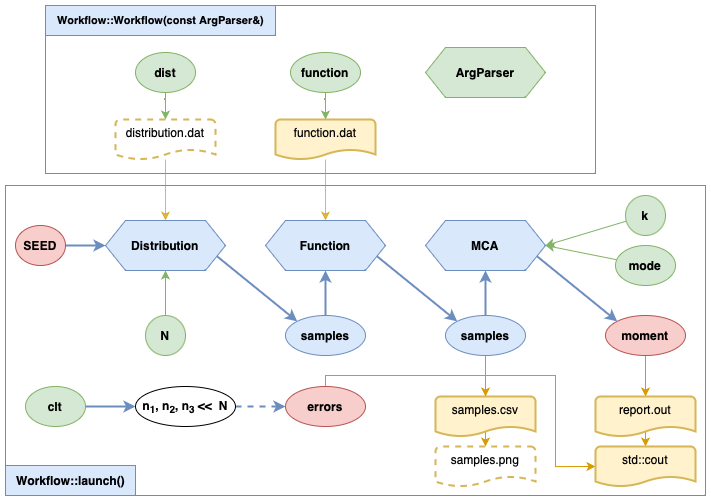
\includegraphics[height=.68\textheight]{img/diag_workflow.png}
    \end{figure}

  \begin{itemize}
    \item \textbf{Distribution:} \texttt{Uniform}, \texttt{Normal}
    \item \textbf{Function:}
        \texttt{CombinedFunction},
        \texttt{MultivariatePolynomial}, \texttt{Polynomial}, \texttt{Linear},
        \texttt{SumExponential}, \texttt{SumLogarithm}
  \end{itemize}

\end{frame}

\begin{frame}{Classes: Function}
    \begin{columns}
        \column{.2\textwidth} {\centering \begin{figure} \centering 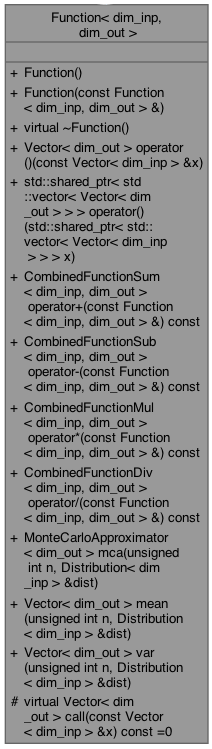
\includegraphics[width=\textwidth]{img/uml_Function.png} \end{figure}}
        \column{.6\textwidth} {\centering \begin{figure} \centering 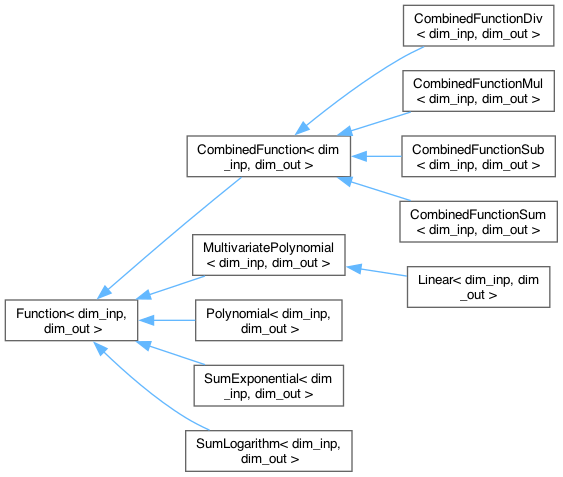
\includegraphics[width=\textwidth]{img/inherit_Function.png} \end{figure}}
        \column{.2\textwidth} {\centering \begin{figure} \centering 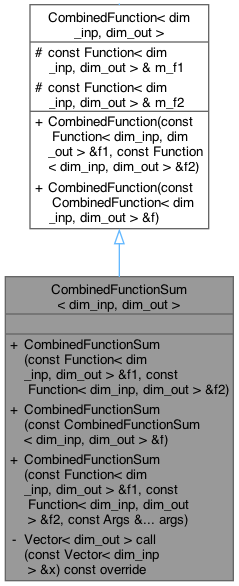
\includegraphics[width=\textwidth]{img/uml_CombinedFunctionSum.png} \end{figure}}
    \end{columns}
\end{frame}

\begin{frame}{Classes: Distribution, Exception, Others}
    \begin{columns}
        \column{.43\textwidth} {
            \centering
            \begin{figure} \centering 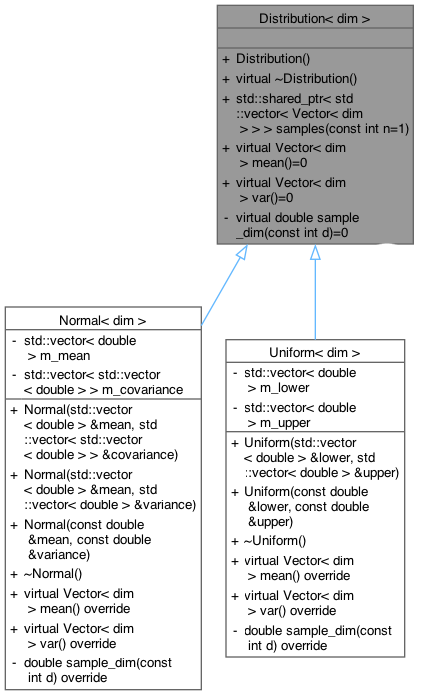
\includegraphics[width=\textwidth]{img/uml_Distributions.png} \end{figure}
        }
        \column{.55\textwidth} {
            \centering
            \begin{figure} \centering 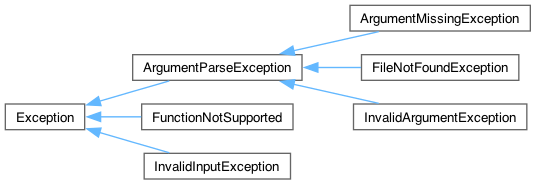
\includegraphics[width=\textwidth]{img/inherit_Exception.png} \end{figure}
            \begin{itemize}
                \item \texttt{Vector}:
                \begin{itemize}
                    \item Storing the elements in a static array
                    \item Connstructors: copy, scalar, standard vector, \texttt{Eigen::VectorXd}
                    \item Operators: assignment, access, stream, scalars, other vectors
                    \item Methods: dot, abs, exp, log, to\_std\_vector
                \end{itemize}
                \item \texttt{MonteCarloApproximator}:
                \begin{itemize}
                    \item Storing samples
                    \item mapping to Eigen matrix
                    \item calculating moments
                \end{itemize}
                \item \texttt{Workflow}:
                \begin{itemize}
                    \item Wrapping up the workflow
                    \item Initializing the function and distribution
                    \item Interacting with IO files
                \end{itemize}
                \item \texttt{ArgParser}:
                \begin{itemize}
                    \item Manipulating and storing the arguments
                \end{itemize}
            \end{itemize}
        }
    \end{columns}
\end{frame}

\begin{frame}{Tests: Vector, Function, Distribution}
    \begin{table}
        \centering
        \textbf{Implemented tests} \\
        \vfill
        \begin{tabular}{|c|l|}
            \hline
            \textbf{Test Name} & \textbf{Description} \\
            \hline
            VectorInitStd & Construct from \texttt{std::vector} \\
            VectorSize & Construct from scalar; Convert to \texttt{std::vector} \\
            VectorPlus & Sum two vectors \\
            VectorMinus & Subtract two vectors \\
            VectorTimes & Multiply two vectors elementwise \\
            VectorDivide & Divide two vectors \\
            VectorDot & Scalar product of two vectors \\
            \hline
            PolynomialEval & Evaluate a \texttt{Polynomial} \\
            MultivariatePolynomialEval & Evaluate a \texttt{MultivariatePolynomial} \\
            LinearEval &  Evaluate a \texttt{Linear} \\
            SumExponentialEval & Evaluate a \texttt{SumExponential} \\
            SumLogarithmEval & Evaluate a \texttt{SumLogarithm} \\
            \hline
            CombinedSum & Sum multiple functions \\
            CombinedDiff & Subtract multiple functions \\
            CombinedProd & Multiply multiple functions \\
            CombineDiv & Divide multiple functions \\
            ComplexCombination & Combined operations on multiple finctions \\
            \hline
            UniformSamples & Check the range of the uniform samples \\
            UniformMean & Check the mean of the uniform samples \\
            UniformVariance & Check the variance of the uniform samples \\
            NormalVariance & Check the variance of the normal samples \\
            \hline
        \end{tabular}
    \end{table}
\end{frame}

\begin{frame}{Tests: MonteCarloApproximator}
    \begin{table}
        \centering
        \textbf{Implemented tests (continued)} \\
        \vfill
        \begin{tabular}{|c|l|}
            \hline
            \textbf{Test Name} & \textbf{Description} \\
            \hline
            Mean & Calculate the mean of a few samples \\
            Var & Calculate the variance of a few samples \\
            Std & Calculate the standard deviation of a few samples \\
            Moment2 & Calculate the second raw moment of a few samples \\
            Moment3 & Calculate the third raw moment of a few samples \\
            Moment4 & Calculate the fourth raw moment of a few samples \\
            Skewness & Calculate the skewness of a few samples \\
            Kurtosis & Calculate the kurtosis of a few samples \\
            Hyperskewness & Calculate the hyperskewness of a few samples \\
            Hypertailedness & Calculate the hypertailedness of a few samples \\
            \hline
        \end{tabular}
    \end{table}

    \begin{table}
        \centering
        \textbf{Tests to be added} \\
        \vfill
        \begin{tabular}{|c|l|}
            \hline
            \textbf{Class} & \textbf{Behaviour} \\
            \hline
            Vector & The scalar operators \\
            Vector & The assignment operators \\
            Vector & Element-wise methods: \textbf{abs}, \textbf{exp}, \textbf{log} \\
            Function & \textbf{mca}, \textbf{mean}, and \textbf{var} for a simple function \\
            Function & Construct from coefficients \\
            \hline
        \end{tabular}
    \end{table}
\end{frame}

\begin{frame}{Features and Example}
    \begin{block}{\$ build/main --help}
        \texttt{USAGE: build/main --function (input-function-file) [-k (order)] [--mode (moment-mode)] [--dist (sample-distribution)] [--n (n-samples)] [--output (output-directory)] [--plot plot-samples] [--clt (show-clt-convergence)]}
    \end{block}
    \begin{columns}[T]
        \column{.2\textwidth} {
            \centering
            \begin{figure} \centering 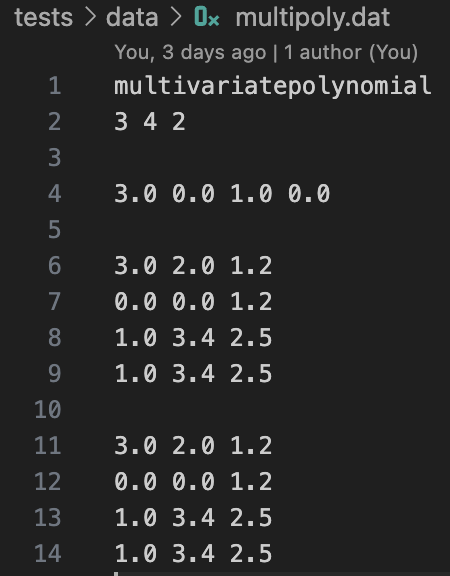
\includegraphics[height=.35\textheight]{img/usage_multipoly.png} \end{figure}
        }
        \column{.5\textwidth} {
            \centering
            \begin{figure} \centering 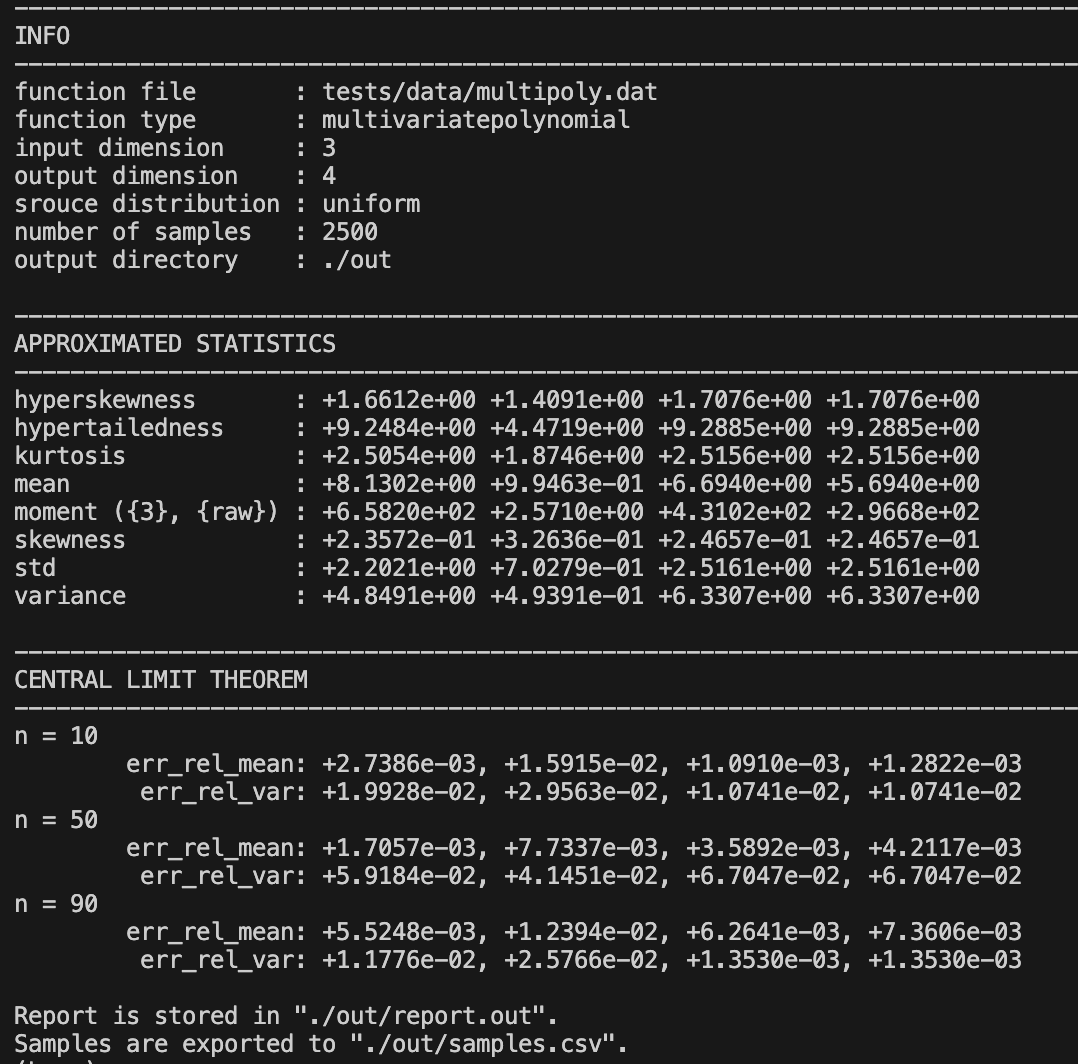
\includegraphics[width=\textwidth]{img/usage_stdout.png} \end{figure}
        }
        \column{.3\textwidth} {
            \begin{figure} \centering 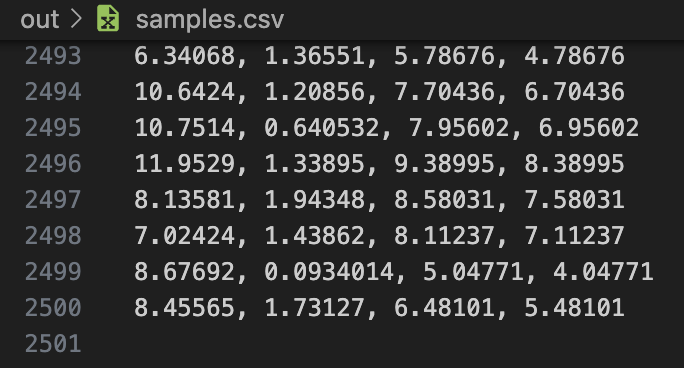
\includegraphics[width=\textwidth]{img/usage_samples.png} \end{figure}
            \footnotesize Output files:
            \begin{itemize}
                \footnotesize
                \item \texttt{out/report.out}: Same information as standard output (except CLT)
                \item \texttt{out/samples.csv}: The random samples from the function distribution
                \item \texttt{out/samples.png} (to be implemented)
            \end{itemize}
        }
    \end{columns}

\end{frame}

\begin{frame}{Remarks and Prospect}

    \textbf{Fixed dimensions:}
    \begin{itemize}
        \item The codes can be used as a static library.
        \item Since the input and output dimensions are templated, the compiled executable is always limited to a set of pre-defined dimensions.
        \item This behaviour can be changed by implementing dynamic memory allocation for \texttt{Vector}, \texttt{Function}, and \texttt{Workflow}.
    \end{itemize}

    \vfill

    \textbf{Data types and memory allocation:}
    \begin{itemize}
        \item The data type of \texttt{Vector} (currently \texttt{double}) should be templated.
        \item Since the size of the vectors (e.g., \texttt{n\_samples}) are always fixed, the code can benefit from static arrays (\texttt{std::array}) instead of vectors (\texttt{std::vector}).
    \end{itemize}

    \vfill

    \textbf{Next steps:}
    \begin{itemize}
        \item The configurations of the source distribution can be loaded from an input file, similar to \texttt{Function}.
        \item Histograms of the generated samples and convergence plots for the Central Limit Theorem can be added to the outputs.
    \end{itemize}


\end{frame}

\end{document}
